\documentclass[11pt,a4paper]{article}

\usepackage[margin=1in]{geometry}
\usepackage{graphicx}
\usepackage{booktabs}
\usepackage{amsmath}
\usepackage{hyperref}
\usepackage{float}
\usepackage{caption}
\usepackage{subcaption}

\title{Shape vs.\ Appearance: Comparing DINOv2 and YOLOv8 on Original and Hollow Contour CIFAR-10 Images}
\author{}
\date{}

\begin{document}
\maketitle

\begin{abstract}
We investigate how well vision models can classify images using only shape outlines (Canny edge contours) compared to full-color originals. We compare two architectures---DINOv2 (a self-supervised Vision Transformer) and YOLOv8n-cls (a lightweight CNN classifier)---on CIFAR-10 in both its original form and a contour-only variant. Both models achieve $\sim$96\% accuracy on original images, but diverge sharply on contours: YOLOv8n retains 70.4\% accuracy while DINOv2 drops to 51.6\%. This suggests that fine-tuned CNNs can more effectively leverage shape information alone, whereas DINOv2's frozen self-supervised features rely more heavily on texture and color.
\end{abstract}

\section{Introduction}

A long-standing question in visual recognition is the relative importance of shape versus texture in how neural networks classify objects~\cite{geirhos2019imagenet}. Human perception is strongly shape-biased, yet convolutional neural networks have been shown to rely more on local texture cues. Self-supervised Vision Transformers such as DINO~\cite{caron2021emerging} have been reported to develop more shape-aware representations, attending to object boundaries even without explicit supervision.

In this study, we test this claim empirically by removing all texture and color information from CIFAR-10 images, leaving only Canny edge contours (hollow outlines). We then measure classification performance of two contrasting architectures:

\begin{itemize}
    \item \textbf{DINOv2} (ViT-S/14): A frozen self-supervised Vision Transformer with a linear classification head trained on the target data.
    \item \textbf{YOLOv8n-cls}: A lightweight convolutional classifier, fully fine-tuned from pretrained ImageNet weights.
\end{itemize}

\section{Method}

\subsection{Dataset Preparation}

We use CIFAR-10 (50,000 training images, 10,000 test images across 10 classes). For each image, we generate a contour version by:
\begin{enumerate}
    \item Converting to grayscale.
    \item Applying Canny edge detection (thresholds: 100, 200).
    \item Saving the binary edge map as a PNG.
\end{enumerate}

Both original and contour images are resized to $224 \times 224$ at inference/training time. Figure~\ref{fig:showcase} shows example pairs.

\begin{figure}[H]
    \centering
    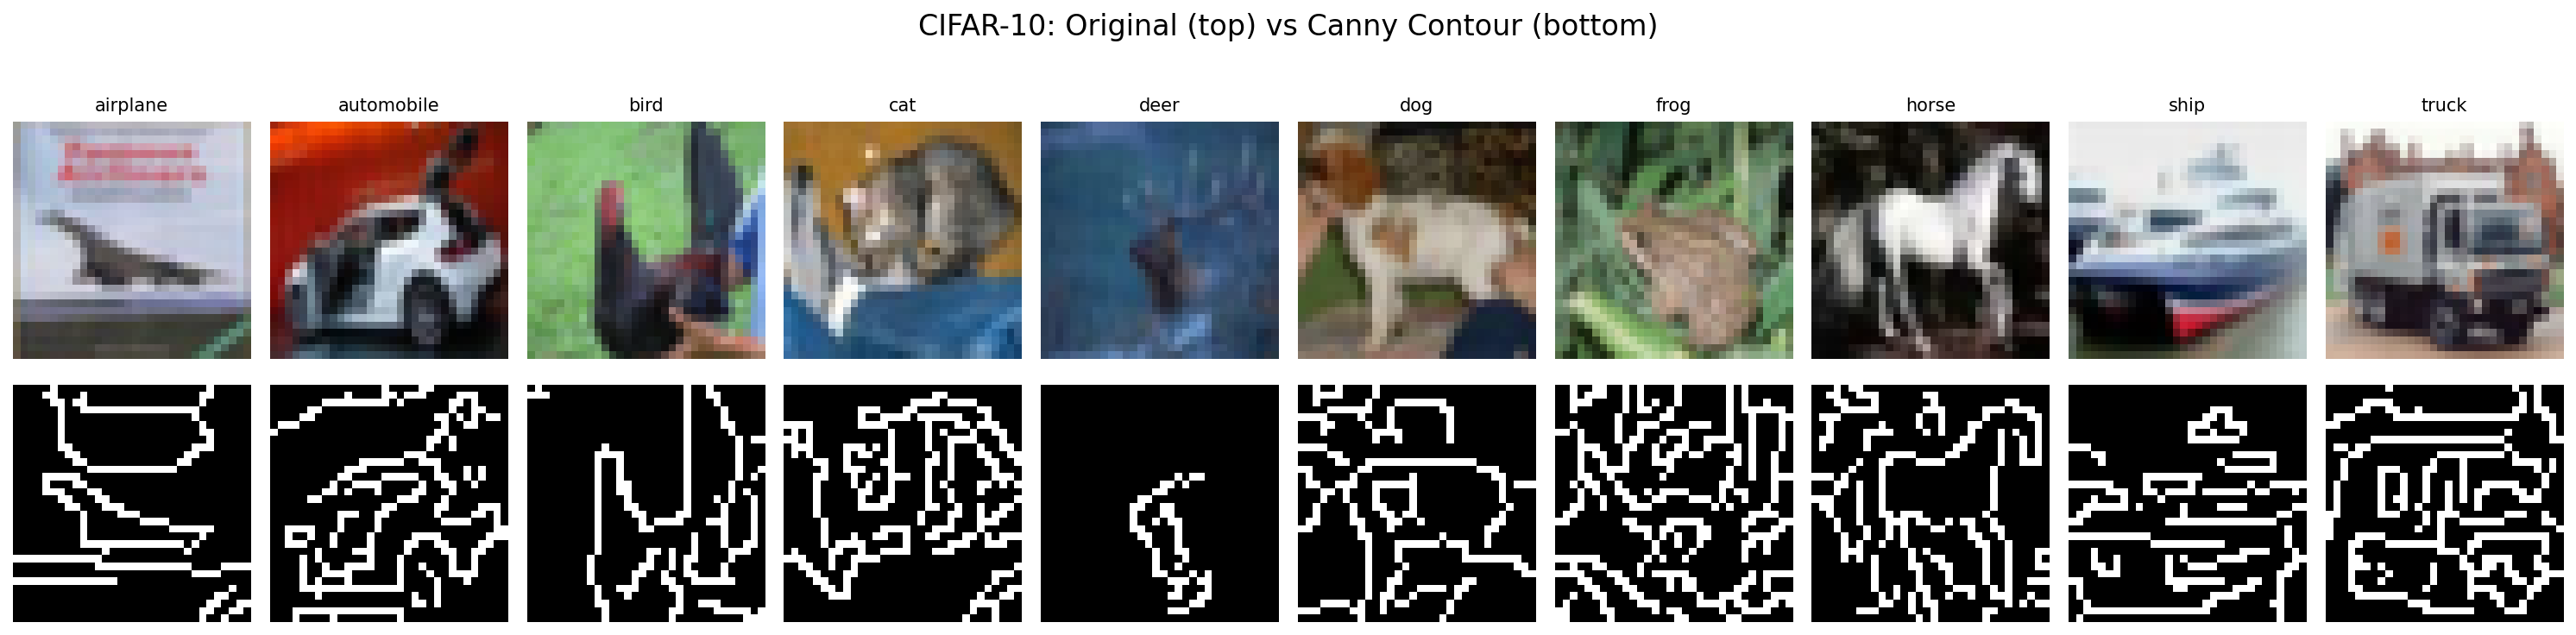
\includegraphics[width=\textwidth]{../results/showcase_grid.png}
    \caption{Sample images from each CIFAR-10 class. Top row: originals. Bottom row: Canny edge contours.}
    \label{fig:showcase}
\end{figure}

\subsection{DINOv2 Setup}

We use the \texttt{dinov2\_vits14} model from the official DINOv2 release. The ViT-S/14 backbone is frozen, and we train only a linear classifier (384-dim $\rightarrow$ 10 classes) on top of the \texttt{[CLS]} token output. Training runs for 100 epochs with the Adam optimizer (lr = $1\times10^{-3}$) and cosine annealing, batch size 256.

\subsection{YOLOv8n-cls Setup}

We use the Ultralytics YOLOv8n-cls model, pretrained on ImageNet. All layers are fine-tuned for 30 epochs with the AdamW optimizer (auto-tuned learning rate), batch size 256, image size $224 \times 224$.

\subsection{Hardware}

All experiments were run on a single NVIDIA RTX 6000 Ada Generation (48 GB) with PyTorch 2.6 and CUDA 12.4.

\section{Results}

\subsection{Overall Accuracy}

\begin{table}[H]
    \centering
    \caption{Test accuracy (\%) on CIFAR-10.}
    \label{tab:accuracy}
    \begin{tabular}{lcc}
        \toprule
        \textbf{Model} & \textbf{Original} & \textbf{Contour} \\
        \midrule
        DINOv2 (ViT-S/14, frozen + linear) & 95.89 & 51.59 \\
        YOLOv8n-cls (fine-tuned) & 96.02 & 70.38 \\
        \bottomrule
    \end{tabular}
\end{table}

Both models perform comparably on original images ($\sim$96\%). However, when texture and color are removed, YOLOv8n retains significantly more performance (70.4\%) than DINOv2 (51.6\%)---a gap of nearly 19 percentage points.

\begin{figure}[H]
    \centering
    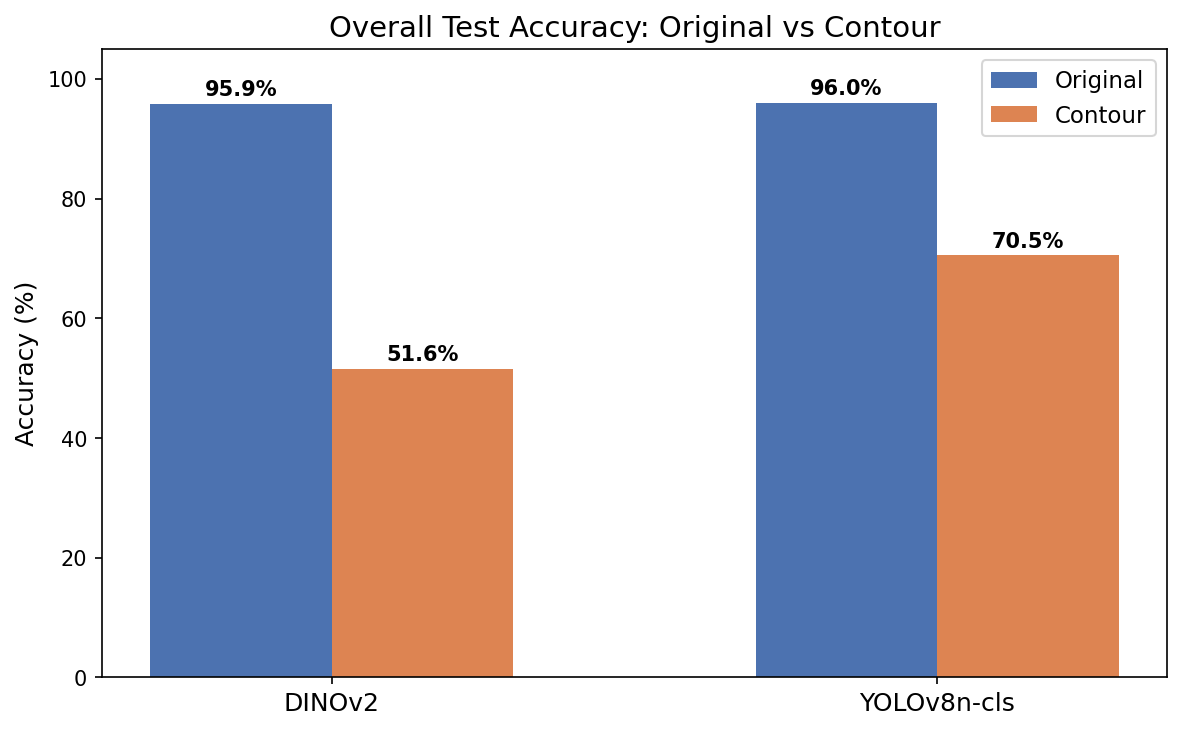
\includegraphics[width=0.7\textwidth]{../results/accuracy_comparison.png}
    \caption{Overall accuracy comparison across models and input variants.}
    \label{fig:accuracy}
\end{figure}

\subsection{Per-Class Analysis}

Figure~\ref{fig:perclass} breaks down accuracy by class. On contour images, YOLO consistently outperforms DINO across all classes. Notably:
\begin{itemize}
    \item Classes with distinctive shapes (\textit{ship}, \textit{airplane}, \textit{truck}) retain relatively high accuracy for both models.
    \item Classes with less distinctive contours (\textit{cat}, \textit{deer}, \textit{dog}) suffer the most, especially for DINO.
\end{itemize}

\begin{figure}[H]
    \centering
    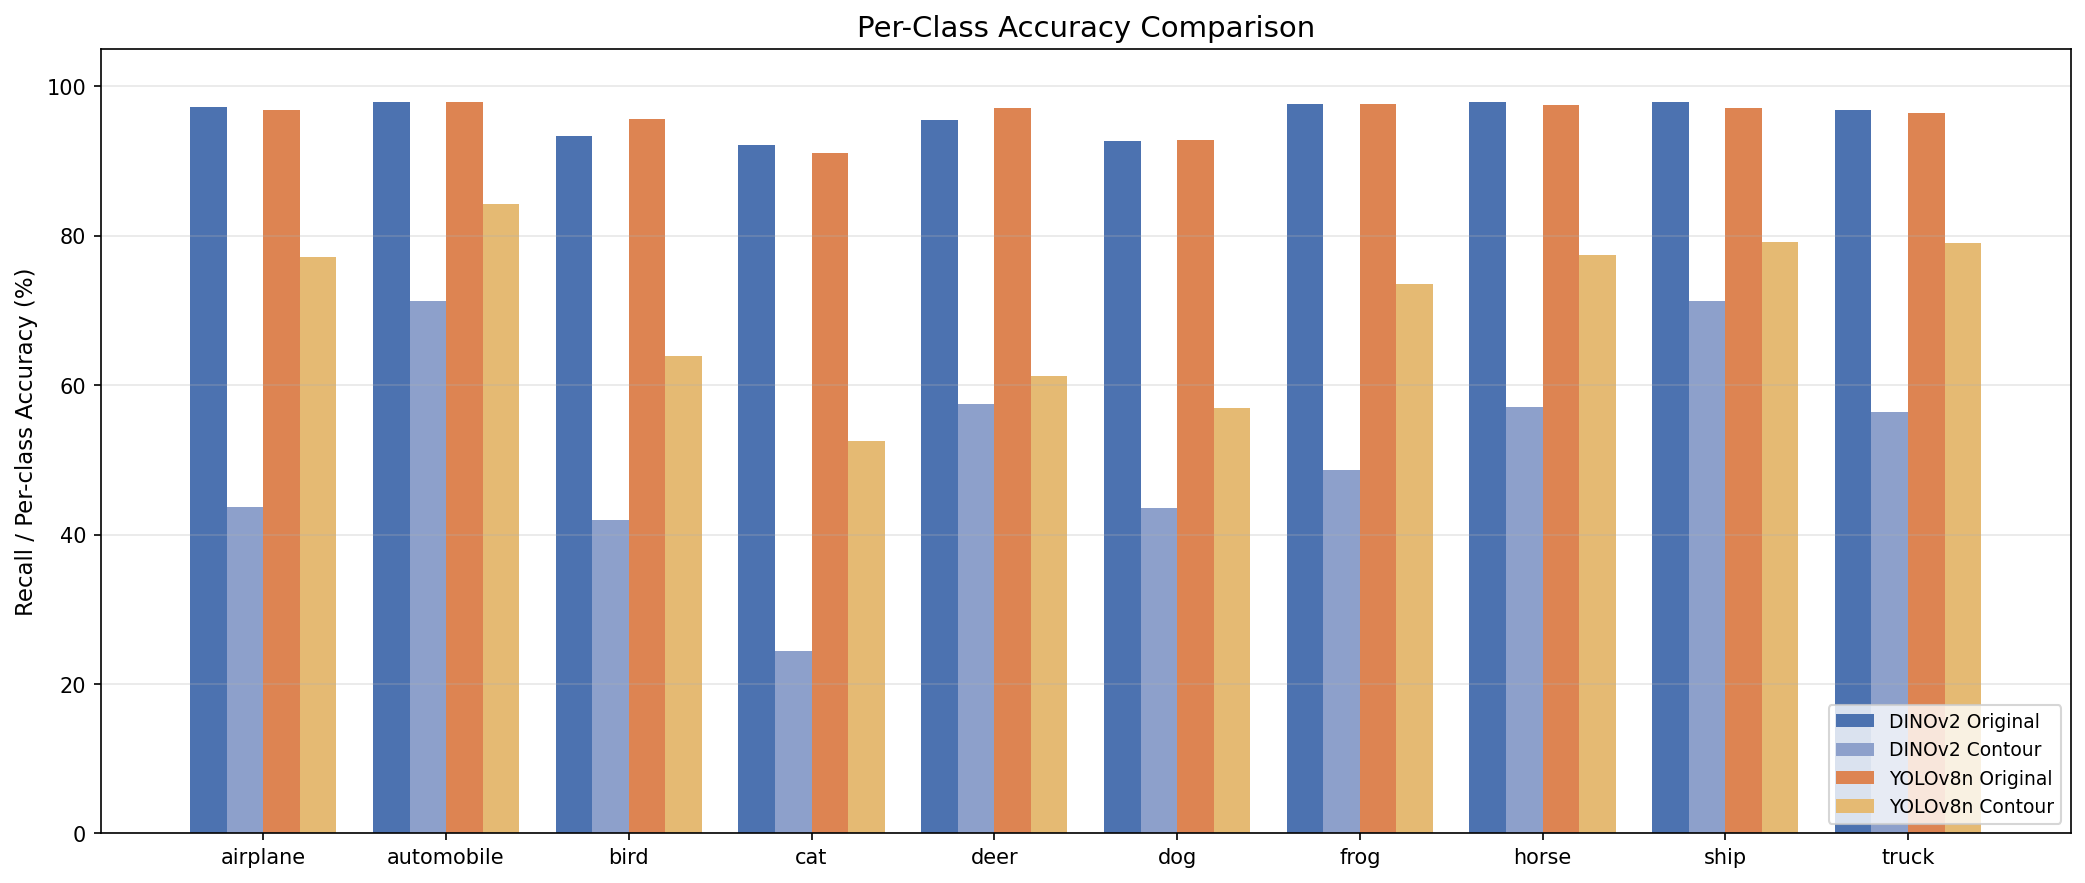
\includegraphics[width=\textwidth]{../results/per_class_accuracy.png}
    \caption{Per-class accuracy (recall) for all four configurations.}
    \label{fig:perclass}
\end{figure}

\subsection{Confusion Matrices}

Figure~\ref{fig:cm} shows normalized confusion matrices. On contour images, DINO exhibits widespread confusion, particularly misclassifying animals as \textit{dog}. YOLO's contour confusion is more structured, with most errors occurring between visually similar categories (e.g., \textit{cat} $\leftrightarrow$ \textit{dog}, \textit{automobile} $\leftrightarrow$ \textit{truck}).

\begin{figure}[H]
    \centering
    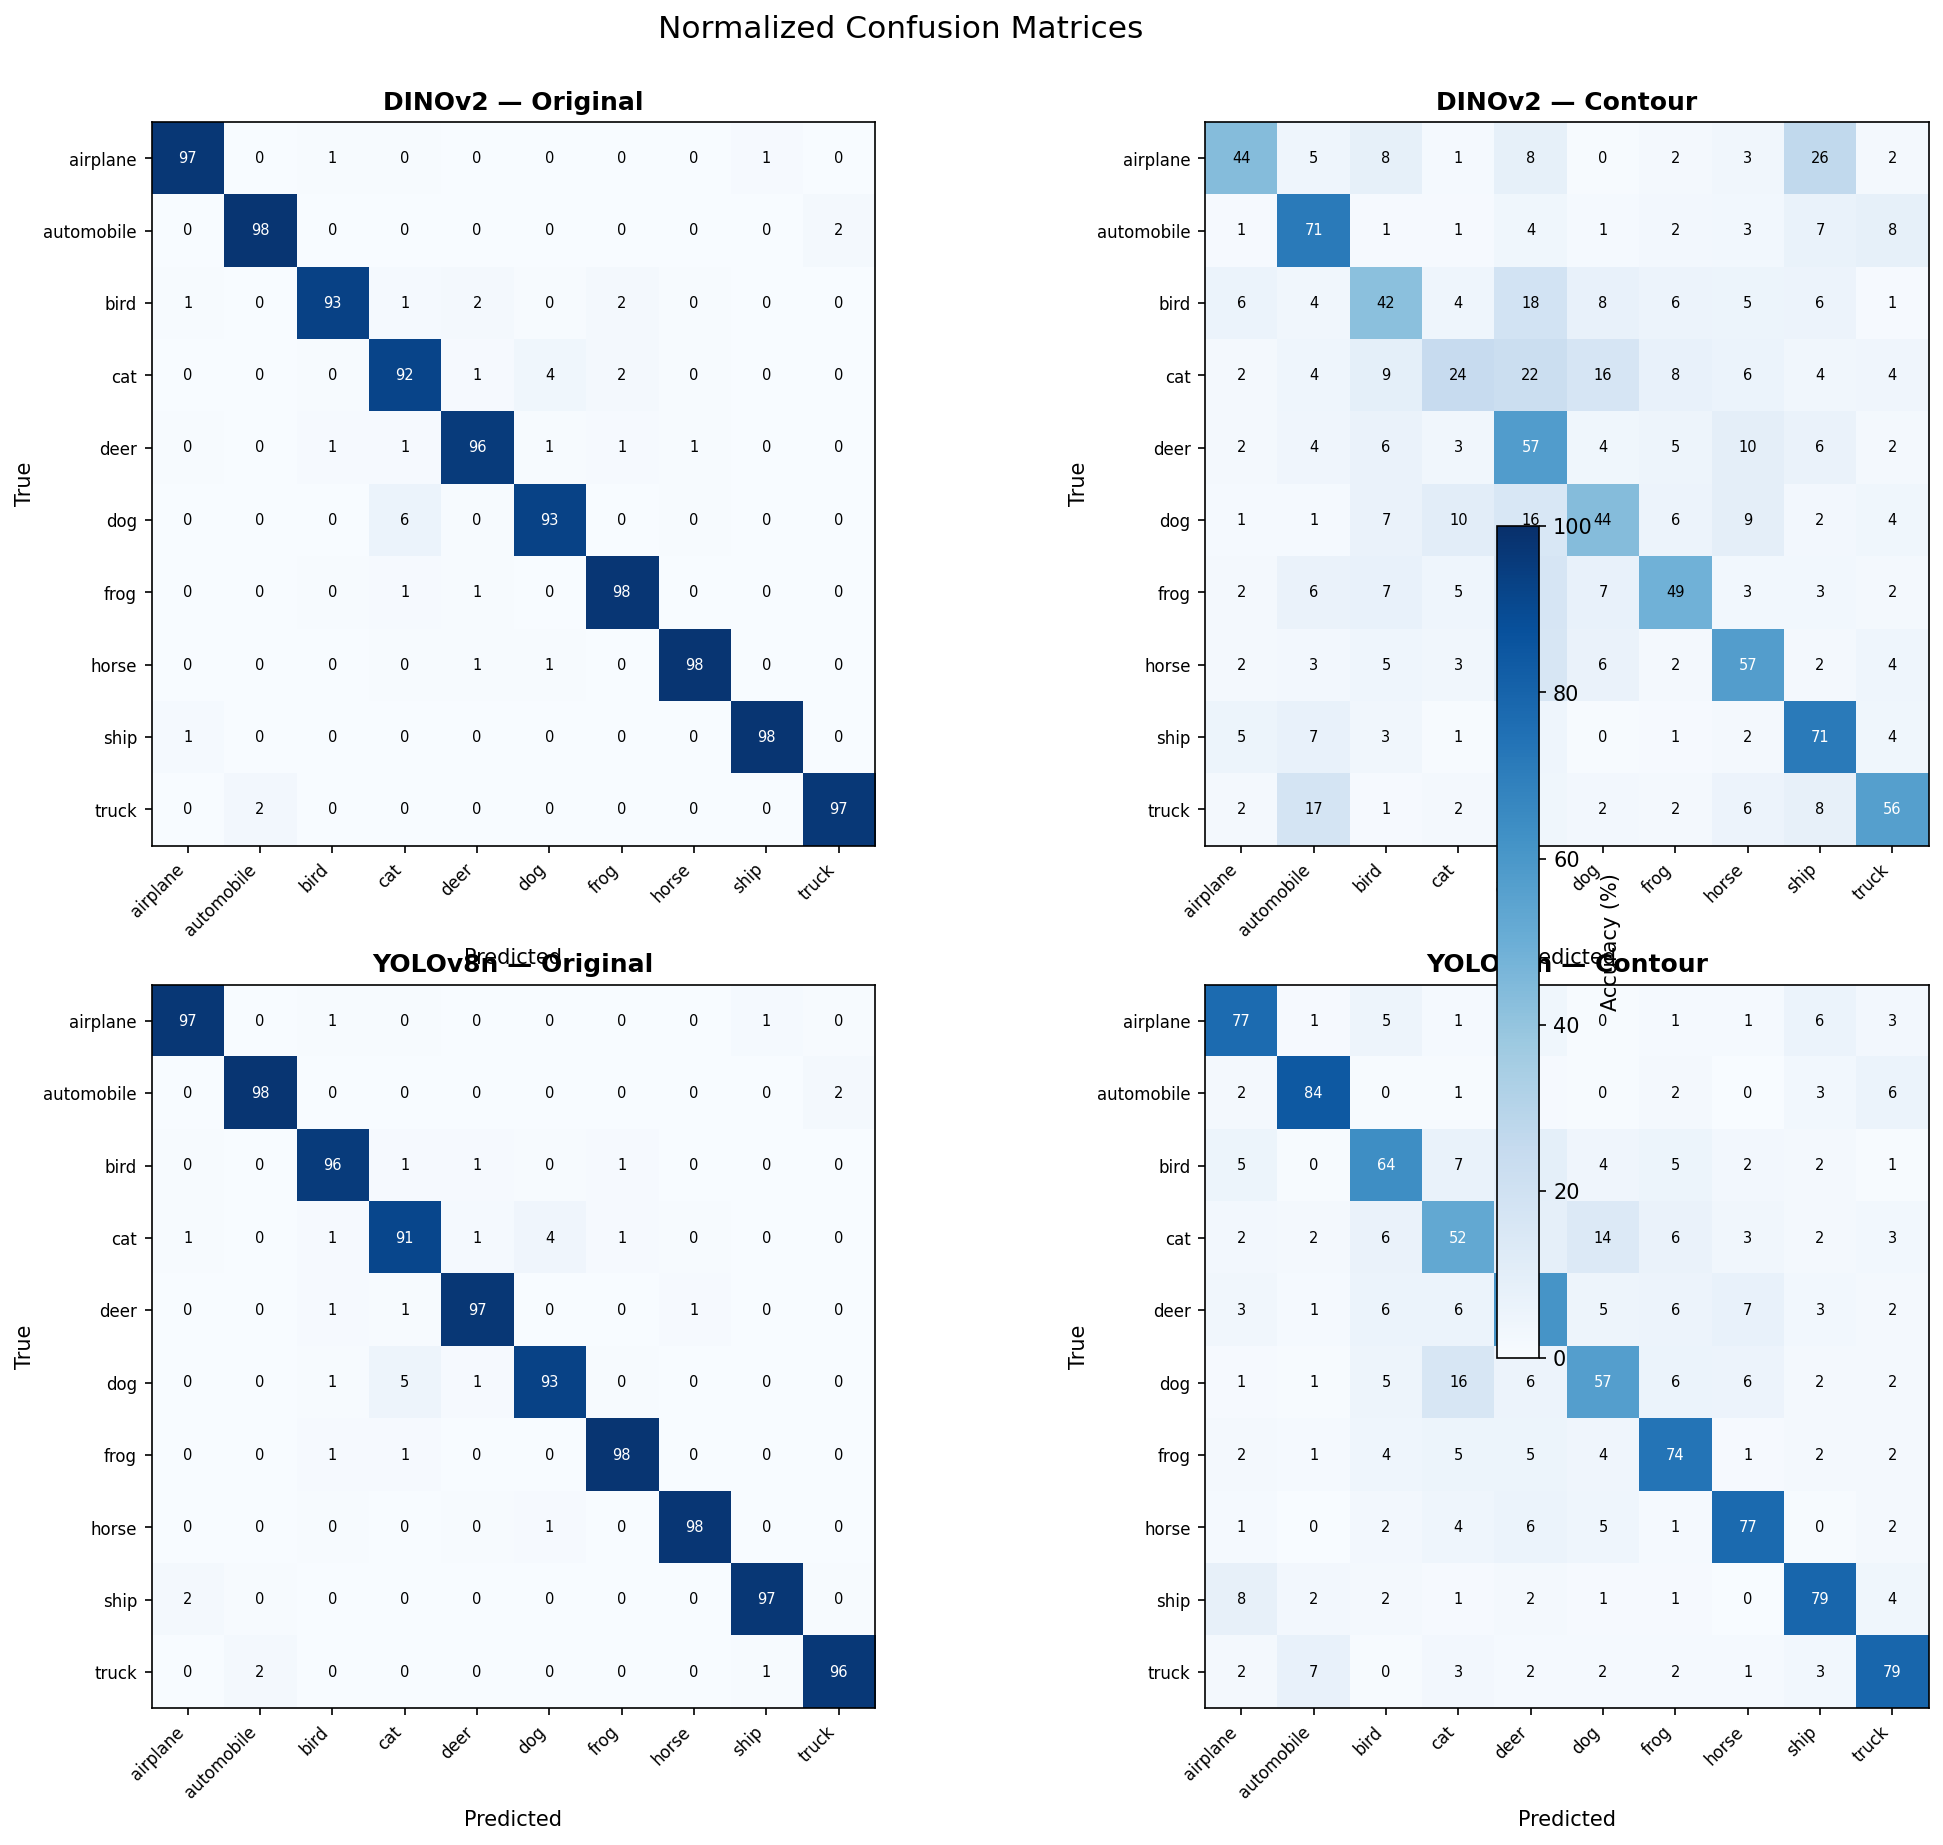
\includegraphics[width=\textwidth]{../results/confusion_matrices.png}
    \caption{Normalized confusion matrices for all four configurations.}
    \label{fig:cm}
\end{figure}

\subsection{Training Curves}

Figure~\ref{fig:curves} shows the training loss and validation accuracy over epochs. YOLO converges faster on original images and achieves steady improvement on contours over all 30 epochs. DINOv2's linear probe converges quickly but plateaus at a much lower level for contour inputs.

\begin{figure}[H]
    \centering
    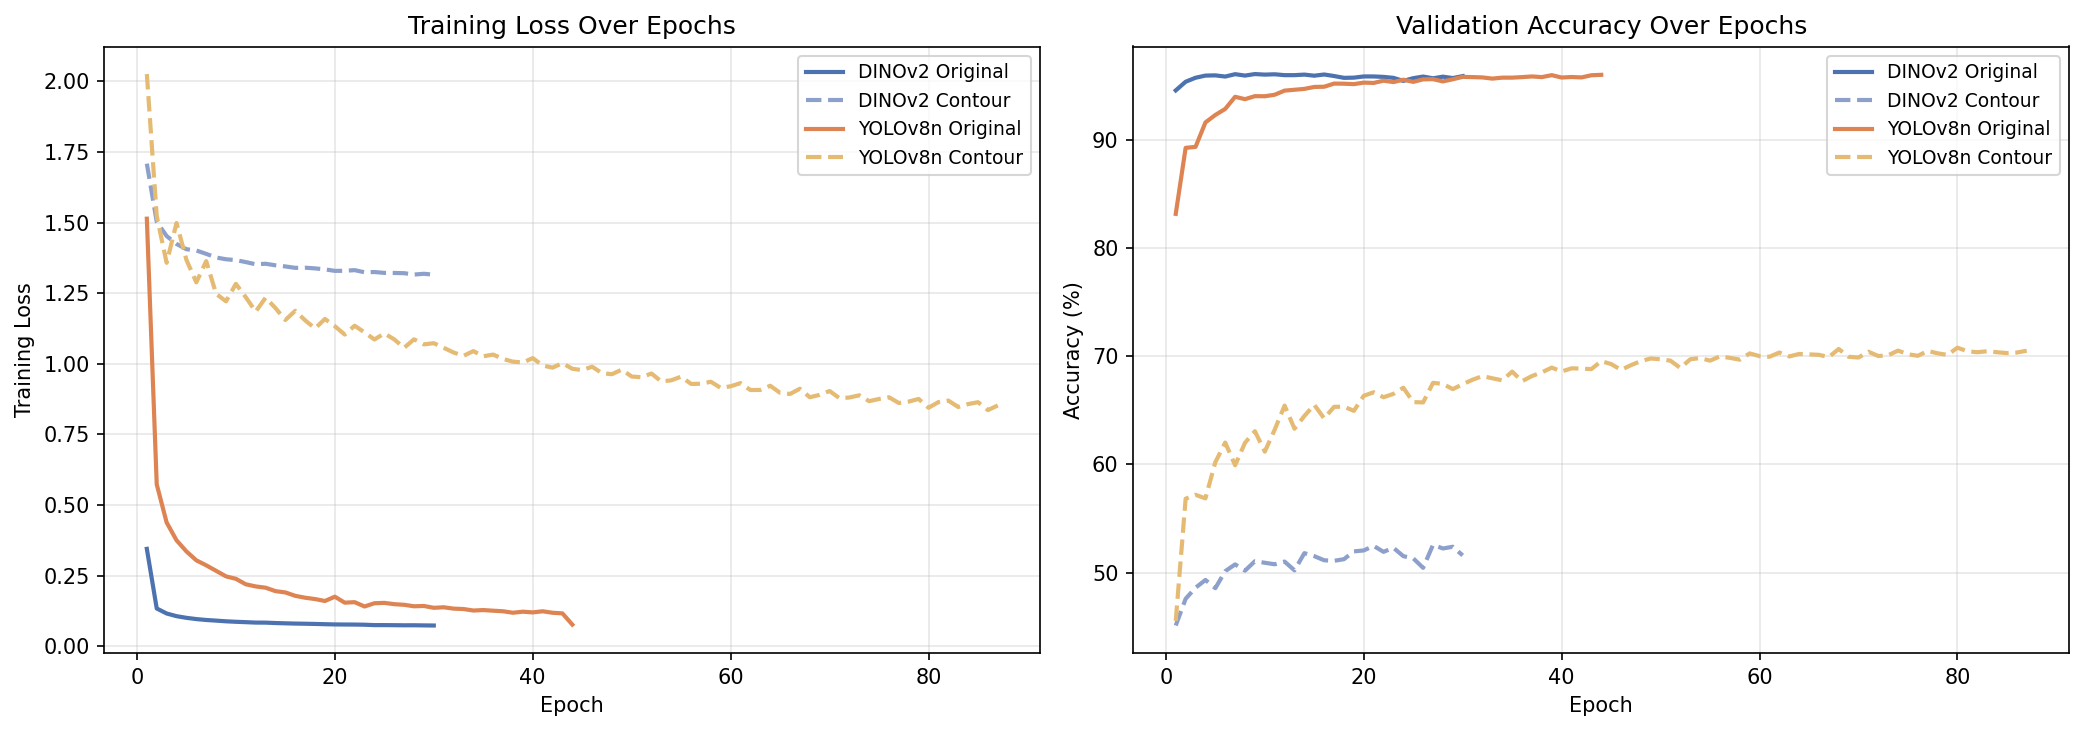
\includegraphics[width=\textwidth]{../results/training_curves.png}
    \caption{Training loss (left) and validation accuracy (right) over epochs.}
    \label{fig:curves}
\end{figure}

\section{Discussion}

\subsection{Why Does YOLO Outperform DINO on Contours?}

The key difference lies in the training paradigm:

\begin{itemize}
    \item \textbf{DINOv2 (frozen backbone + linear probe)}: The features were learned via self-supervised pretraining on natural images rich in texture and color. When these cues are removed, the frozen representations may not encode the remaining shape information in a linearly separable way. The model cannot adapt its internal representations to the contour domain.

    \item \textbf{YOLOv8n (full fine-tuning)}: All layers are updated during training, allowing the network to adapt its low-level and mid-level features specifically for edge/contour patterns. The convolutional inductive bias (local receptive fields, translation equivariance) may also be better suited to processing sparse edge maps.
\end{itemize}

\subsection{Implications}

\begin{enumerate}
    \item \textbf{Frozen SSL features are domain-sensitive}: DINOv2's impressive general-purpose representations degrade substantially when the input distribution shifts from natural images to binary edge maps. Fine-tuning the backbone (or using adapters) would likely close the gap.

    \item \textbf{Shape alone is partially sufficient}: At 70\% accuracy, YOLO demonstrates that Canny edge contours retain meaningful classification signal, even at CIFAR-10's low $32\times32$ native resolution. However, the $\sim$26\% drop from original suggests that texture and color remain important complementary cues.

    \item \textbf{Architecture matters less than adaptation}: Both models achieve $\sim$96\% on originals, but the ability to adapt to a new input domain (contours) is determined by whether the model can update its features, not by whether it is a ViT or CNN.
\end{enumerate}

\section{Conclusion}

We compared DINOv2 and YOLOv8n-cls on classifying CIFAR-10 images in their original form and as Canny edge contours. While both models achieve $\sim$96\% on originals, YOLOv8n significantly outperforms DINOv2 on contours (70.4\% vs.\ 51.6\%). The primary factor is not architecture (ViT vs.\ CNN) but training strategy: full fine-tuning allows YOLO to adapt to the contour domain, while DINOv2's frozen features---optimized for natural images---fail to represent shape-only inputs effectively. Future work could explore fine-tuning the DINOv2 backbone, using adapter layers, or testing on higher-resolution contour datasets.

\begin{thebibliography}{9}
\bibitem{geirhos2019imagenet}
R.~Geirhos, P.~Rubisch, C.~Michaelis, M.~Bethge, F.~A.~Wichmann, and W.~Brendel,
``ImageNet-trained CNNs are biased towards textures; increasing shape bias improves accuracy and robustness,''
in \textit{Proc.\ ICLR}, 2019.

\bibitem{caron2021emerging}
M.~Caron, H.~Touvron, I.~Misra, H.~J{\'e}gou, J.~Mairal, P.~Bojanowski, and A.~Joulin,
``Emerging properties in self-supervised vision transformers,''
in \textit{Proc.\ ICCV}, 2021.
\end{thebibliography}

\end{document}
